% \begin{frame}{Tổng quan thị giác máy tính}
%     \begin{columns}
%         \begin{column}{0.5\textwidth}
%             \textbf{Các bài toán cơ bản:}
%             \begin{itemize}
%                 \item Phân loại ảnh
%                 \item Nhận diện đối tượng
%                 \item Phân đoạn ảnh
%                 \item Khôi phục ảnh:
%                 \begin{itemize}
%                     \item Denoising
%                     \item Deblurring
%                     \item Super-resolution
%                 \end{itemize}
%             \end{itemize}
%         \end{column}
%         \begin{column}{0.5\textwidth}
%             \begin{figure}
%                 \centering
%                 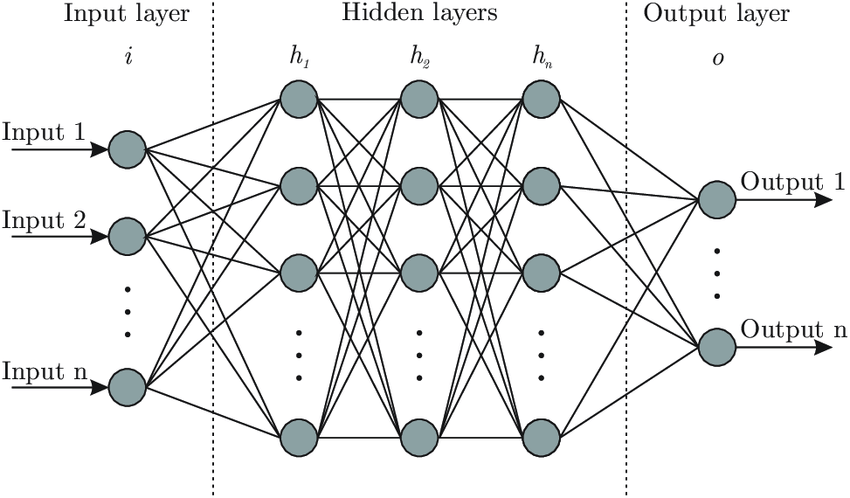
\includegraphics[width=0.8\linewidth]{images/ANN.png}
%                 \caption{Mạng nơ-ron nhân tạo}
%             \end{figure}
%         \end{column}
%     \end{columns}
% \end{frame}

% \begin{frame}{Mạng nơ-ron tích chập (CNN)}
%     \begin{columns}
%         \begin{column}{0.5\textwidth}
%             \textbf{Thành phần chính:}
%             \begin{itemize}
%                 \item \textbf{Lớp tích chập:} Trích xuất đặc trưng
%                 \item \textbf{Lớp pooling:} Giảm kích thước
%                 \item \textbf{ReLU:} Hàm kích hoạt phi tuyến
%                 \item \textbf{Fully connected:} Phân loại
%             \end{itemize}
            
%             \vspace{0.3cm}
%             \textbf{ResNet-50:}
%             \begin{itemize}
%                 \item 50 lớp, sử dụng residual blocks
%                 \item Giải quyết vanishing gradient
%                 \item Backbone mạnh mẽ cho nhiều tác vụ
%             \end{itemize}
%         \end{column}
%         \begin{column}{0.5\textwidth}
%             \begin{figure}
%                 \centering
%                 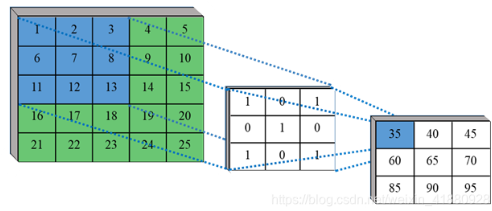
\includegraphics[width=0.9\linewidth]{images/Kernel.png}
%                 \caption{Lớp tích chập}
%             \end{figure}
%             \begin{figure}
%                 \centering
%                 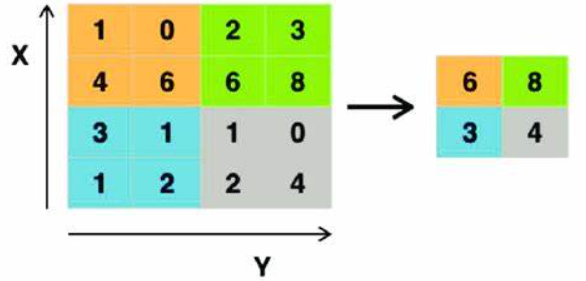
\includegraphics[width=0.7\linewidth]{images/pooling.png}
%                 \caption{Lớp pooling}
%             \end{figure}
%         \end{column}
%     \end{columns}
% \end{frame}

\begin{frame}{Autoencoder (AE)}
    \begin{columns}
        \begin{column}{0.5\textwidth}
            \textbf{Cấu trúc:}
            \begin{itemize}
                \item \textbf{Encoder:} $x \rightarrow z$ (nén)
                \item \textbf{Decoder:} $z \rightarrow \hat{x}$ (tái tạo)
            \end{itemize}
            
            \vspace{0.3cm}
            \textbf{Hàm mất mát:}
            \[
                L(x, \hat{x}) = \| x - \hat{x} \|^2
            \]
            
            \vspace{0.3cm}
            \textbf{Ứng dụng:}
            \begin{itemize}
                \item Khử nhiễu ảnh
                \item Siêu phân giải
                \item Phát hiện bất thường
            \end{itemize}
        \end{column}
        \begin{column}{0.5\textwidth}
            \begin{figure}
                \centering
                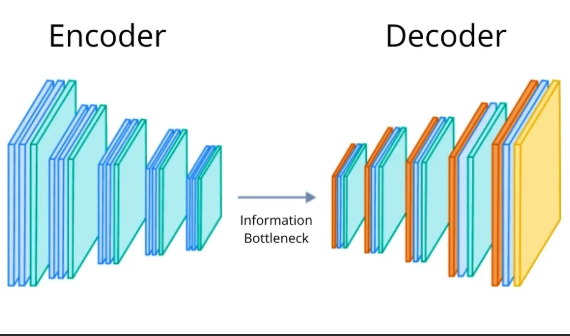
\includegraphics[width=0.9\linewidth]{images/autoencoder.png}
                \caption{Kiến trúc Autoencoder}
            \end{figure}
        \end{column}
    \end{columns}
\end{frame}

% \begin{frame}{Lý thuyết Entropy trong CNN}
%     \begin{block}{Entropy vi phân}
%         Đo lường lượng thông tin của biến ngẫu nhiên:
%         \[
%             H(X) = \mathbb{E}\left[-\log f(X)\right]
%         \]
%     \end{block}
    
%     \begin{block}{Sự thay đổi Entropy qua lớp tích chập}
%         Với bộ lọc $C$ kích thước $p \times q$:
%         \[
%             \Delta H_{\text{conv}} = (l - p + 1)(w - q + 1) \log(|c_{11}|)
%         \]
%         \begin{itemize}
%             \item $|c_{11}| > 1$: Khuếch đại tín hiệu, tăng entropy
%             \item $|c_{11}| < 1$: Làm mịn/nén thông tin, giảm entropy
%         \end{itemize}
%     \end{block}
    
%     \textbf{Ý nghĩa:} Theo dõi entropy giúp hiểu cách mạng xử lý và chuyển hóa thông tin qua các lớp.
% \end{frame}

\begin{frame}{Generative Adversarial Network (GAN)}
    \begin{columns}
        \begin{column}{0.5\textwidth}
            \textbf{Cấu trúc:}
            \begin{itemize}
                \item \textbf{Generator (G):} Sinh ảnh từ noise $z$
                \item \textbf{Discriminator (D):} Phân biệt ảnh thật/giả
                \item Huấn luyện đối kháng
            \end{itemize}

            \textbf{Hàm mất mát đối kháng:}
            \[
                \mathcal{L}_{\text{adv}} = \mathbb{E}[\log D(x)] + \mathbb{E}[\log(1-D(G(z)))]
            \]
        \end{column}
        \begin{column}{0.5\textwidth}
            \begin{figure}
                \centering
                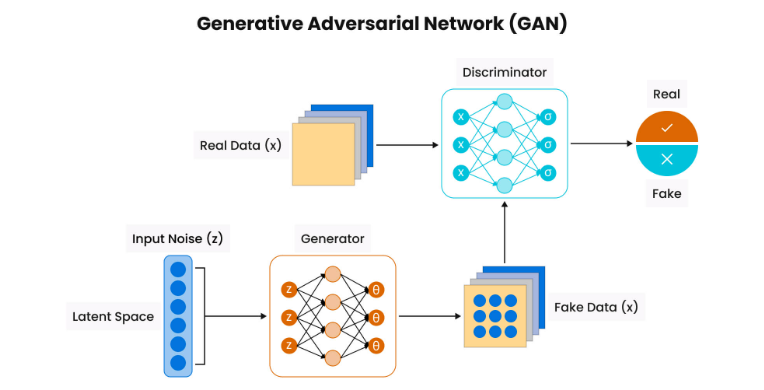
\includegraphics[width=0.9\linewidth]{images/GAN.png}
                \caption{Kiến trúc GAN}
            \end{figure}
        \end{column}
    \end{columns}
    
    \begin{block}{Trong khử nhiễu}
        \begin{itemize}
            \item Generator: Khử nhiễu, khôi phục ảnh sạch
            \item Discriminator: Đánh giá tính chân thực của ảnh khôi phục
            \item Hàm mất mát kết hợp: $\mathcal{L}_G = \lambda_{\text{rec}}\mathcal{L}_{\text{rec}} + \lambda_{\text{adv}}\mathcal{L}_{\text{adv}}$
        \end{itemize}
    \end{block}
\end{frame}

\begin{frame}{Flow-based (FB)}
    \begin{columns}
        \begin{column}{0.5\textwidth}
            \textbf{Ý tưởng:}
            \begin{itemize}
                \item Học ánh xạ khả nghịch $f: x \leftrightarrow z$
                \item $z$ tuân theo phân phối chuẩn
                \item Có thể tính chính xác likelihood
            \end{itemize}
            
            \textbf{Chuỗi biến đổi:}
            \[
                z = f_K \circ f_{K-1} \circ \cdots \circ f_1(x)
            \]
            \textbf{Log-likelihood:}
            \[
                \log p(x) = \log p(z) + \sum_{k=1}^{K} \log \left|\det\left(\frac{\partial f_k}{\partial h_{k-1}}\right)\right|
            \]
        \end{column}
        \begin{column}{0.5\textwidth}
            \begin{figure}
                \centering
                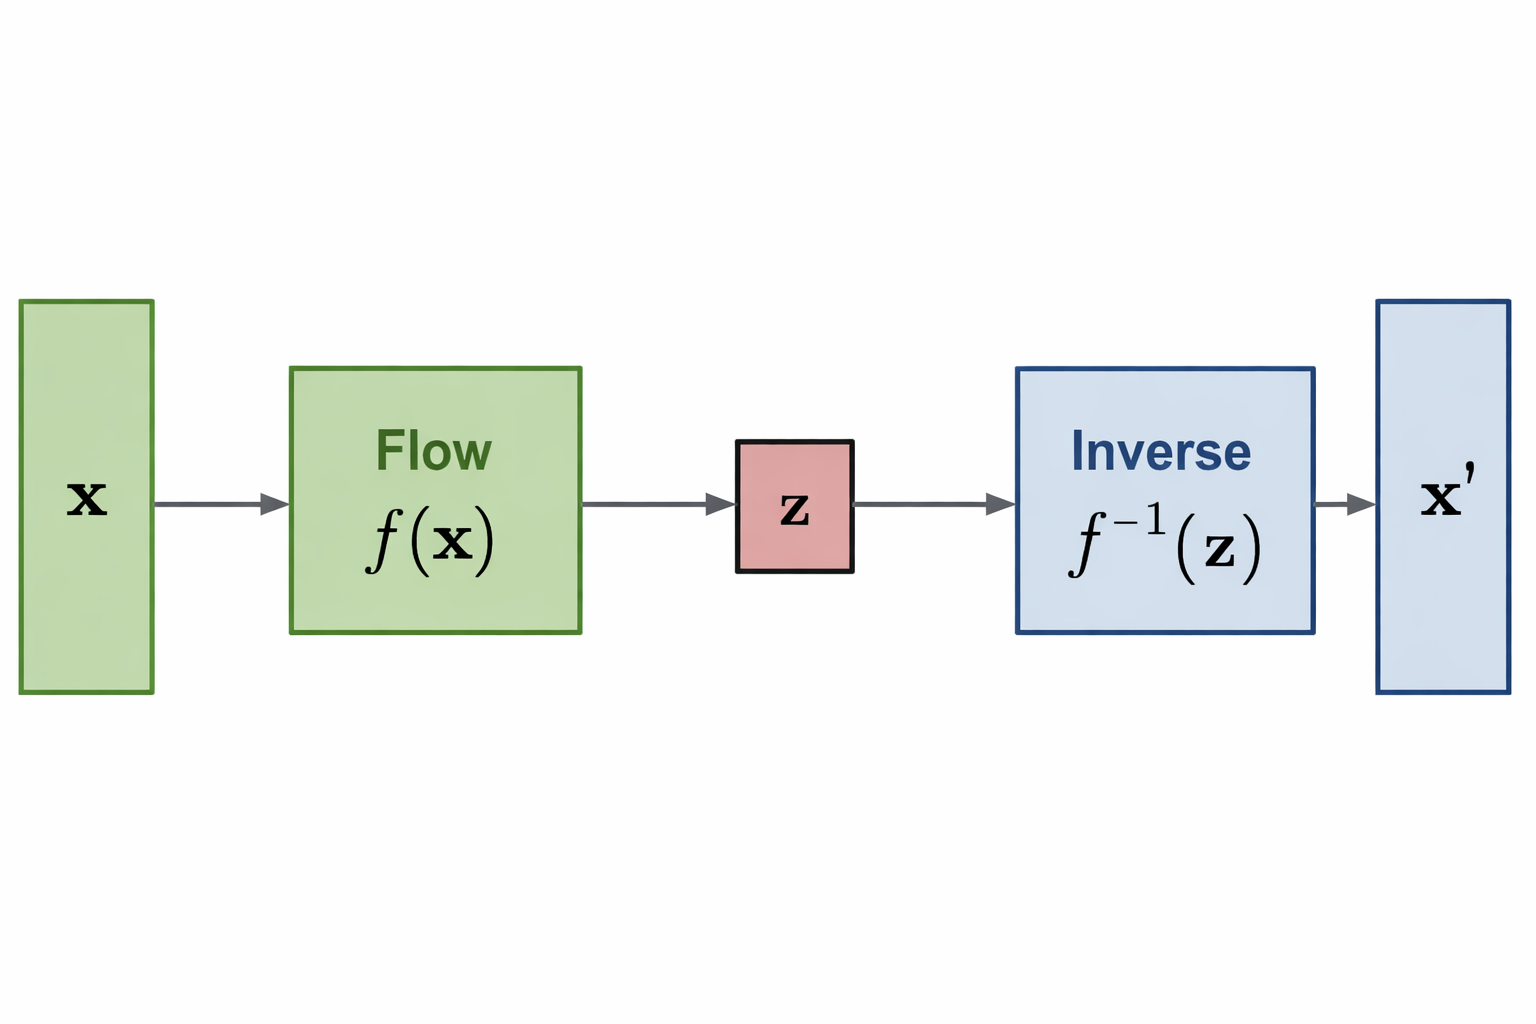
\includegraphics[width=0.5\linewidth]{images/flow.png}
                \caption{Kiến trúc Flow-based}
            \end{figure}
        \end{column}

        
    \end{columns}
    
    % \vspace{0.3cm}
    % \begin{column}{0.7\textwidth}
        % \textbf{Log-likelihood:}
        % \[
        %     \log p(x) = \log p(z) + \sum_{k=1}^{K} \log \left|\det\left(\frac{\partial f_k}{\partial h_{k-1}}\right)\right|
        % \]
    % \end{column}
    % \textbf{Trong khôi phục ảnh:} Mô hình hóa phân phối hậu nghiệm $p(x|y)$ với ảnh quan sát $y$ bị suy giảm.
\end{frame}
